\chapter{Giới thiệu}

\ifpdf
\graphicspath{{Chapter1/Chapter1Figs/PNG/}{Chapter1/Chapter1Figs/PDF/}{Chapter1/Chapter1Figs/}}
\else
\graphicspath{{Chapter1/Chapter1Figs/EPS/}{Chapter1/Chapter1Figs/}}
\fi

Những năm gần đây, \textbf{học tăng cường} (Reinforcement learning) liên tục đạt được những thành tựu quan trọng trong lĩnh vực Trí tuệ nhân tạo (Artificial Intelligence). Những đóng góp nổi bật của phương pháp này bao gồm: tự động điều khiển robot di chuyển, điều khiển mô hình máy bay trực thăng, hệ thống chơi cờ vây... Trong số các thành tựu này, hệ thống chơi cờ vây với khả năng chiến thắng những kỳ thủ hàng đầu thế giới là một cột mốc quan trọng của lĩnh vực Trí tuệ nhân tạo. Dù vậy, học tăng cường không phải là một phương pháp mới được phát triển gần đây. Nền tảng lý thuyết của học tăng cường đã được xây dựng từ những năm 1980. 

Được xây dựng nhằm mô phỏng quá trình học của con người, ý tưởng chính của học tăng cường là tìm cách lựa chọn hành động \textit{tối ưu} để nhận được \textbf{nhiều nhất giá trị điểm thưởng} (Reward). Giá trị điểm thưởng này có ý nghĩa tương tự cảm nhận của con người về môi trường. Khi một đứa trẻ bắt đầu ``học'' về thế giới xung quanh của mình, những cảm giác như đau đớn (ứng với điểm thưởng thấp) hay vui sướng (điểm thưởng cao) chính là mục tiêu cần tối ưu của việc học. Một điểm quan trọng của học tăng cường là nó được xây dựng với ít giả định nhất có thể về môi trường xung quanh. Hệ thống sử dụng học tăng cường (Agent) không cần biết cách thức hoạt động của môi trường để hoạt động. Ví dụ như để điều khiển robot tìm được đi trong mê cung, hệ thống không cần biết mê cung được xây dựng thế nào hay kích thước là bao nhiêu. Việc hạn chế tối đa những ràng buộc về dữ liệu đầu vào của bài toán học tăng cường giúp cho phương pháp này có thể áp dụng vào nhiều bài toán thực tế.

Học tăng cường được xem là một nhánh trong lĩnh vực máy học ngoài hai nhánh: học có giám sát và học không có giám sát. Trong bài toán học có giám sát, dữ liệu thường được gán nhán thủ công sẵn và việc chủ yếu của hệ thống là làm sao dự đoán chính xác các nhãn đó với dữ liệu mới. Các nhãn này có thể xem như là sự hướng dẫn trong quá trình học; tính đúng sai của việc học lúc này có thể được xác định dựa vào kết quả dự đoán của hệ thống và nhãn đúng của dữ liệu. Tiếp theo đối với những bài toán học không có giám sát, dữ liệu học thường không được gán nhãn nên công việc của việc học là phải tự tìm ra được cấu trúc ``ẩn'' bên dưới dữ liệu đó. Khác với hai loại bài toán vừa nêu, trong bài toán học tăng cường, hệ thống \textit{không nhận được nhãn thực sự} (tức hành động tối ưu của tình huống hiện tại) mà chỉ nhận được điểm thưởng từ môi trường. Điểm thưởng lúc này chỉ thể hiện mức độ ``tốt/xấu'' của hành động vừa chọn chứ không nói lên hành động đó có phải là hành động tối ưu hay không. Điểm thưởng này thông thường rất thưa: ta có thể chỉ nhận được điểm thưởng có ý nghĩa (khác không) sau hàng nghìn hành động. Ngoài ra, giá trị điểm thưởng thường là không đơn định và rất nhiễu: cùng một hành động tại cùng một trạng thái, ta có thể nhận được điểm thưởng khác nhau vào hai thời điểm khác nhau. Đây cũng chính là những khó khăn cơ bản của bài toán học tăng cường.

Các trò chơi điện tử thường hay có điểm số mà người chơi cần phải tối ưu hoá. Đặc điểm này trùng với yêu cầu của bài toán học tăng cường, vì vậy các trò chơi này cũng chính là những ứng dụng tự nhiên nhất của phương pháp học tăng cường. Trong luận văn này, chúng em áp dụng phương pháp học tăng cường nhằm xây dựng \textbf{hệ thống tự động chơi các game} trên hệ máy Atari. Dữ liệu đầu vào của hệ thống chỉ bao gồm các frame ảnh RGB cùng với điểm số hiện tại. Từ hình ảnh thô này, hệ thống cần tìm cách chơi sao cho điểm số cuối màn chơi (Episode) là lớn nhất có thể. Hệ thống hoàn toàn không biết quy luật của game trước khi bắt đầu quá trình học mà phải tự tìm hiểu quy luật và chiến thuật chơi tối ưu. Lý do luận văn sử dụng game của máy Atari là vì các game này có quy luật chơi tương đối đơn giản nhưng lại rất đa dạng. Mỗi màn chơi thường có độ dài vừa phải (từ 2 - 15 phút) và số hành động có ý nghĩa không quá nhiều (18 hành động). Ngoài ra, các trò chơi này có thể được giả lập trên máy vi tính với tốc độ cao, giúp quá trình học được tăng tốc.

\begin{figure}
	\centering
	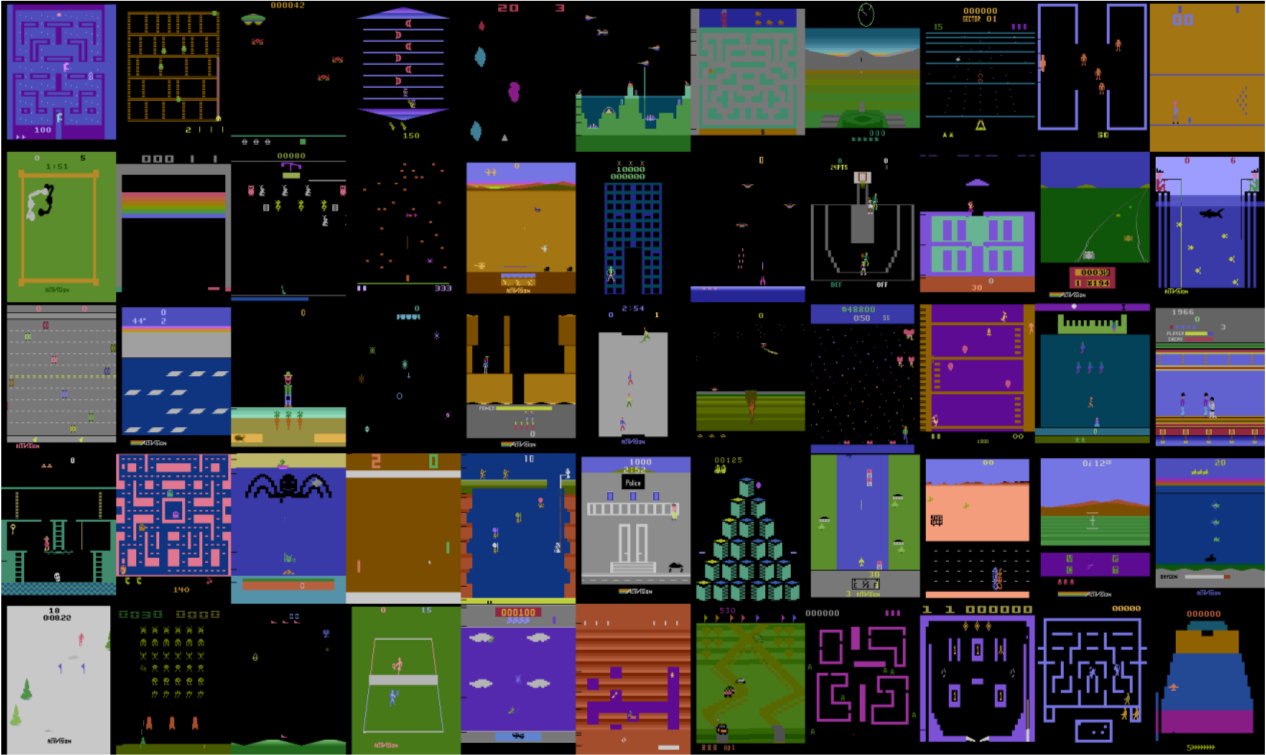
\includegraphics[width=\textwidth]{ale_55_games}
	\caption{Hình ảnh các game trên hệ máy Atari}
	\label{Ale55Games}
\end{figure}

Một số khó khăn trước mắt có thể thấy ở bài toán tự động chơi game bao gồm:
\begin{itemize}
	\item Hệ thống không được cung cấp luật chơi của game. Chính vì thế nó cũng không thể biết được hành động nào nên làm hoặc không nên làm ứng với từng tình huống cụ thể.
	\item Dữ liệu đầu vào là hình ảnh RGB có kích thước $210\times160$. Để học được một chiến thuật chơi đơn giản thì hệ thống cũng phải chơi ``thử và sai'' một số lượng lớn màn chơi (có thể lên đến 10000 frame). Vì vậy, lượng dữ liệu đầu vào cần phải xử lý là rất lớn.
	\item Các game có hình ảnh, nội dung rất khác nhau. Để có thể học cách chơi của nhiều game khác nhau thì thuật toán học phải mang tính tổng quát cao, không sử dụng các tính chất riêng biệt của từng game.
	\item Để đạt được điểm số cao (ngang hoặc hơn điểm số của con người) thì phải tìm được chiến thuật chơi mang tính lâu dài. Những phương pháp tham lam, lựa chọn hành động để đạt điểm tối đa trong tương lai gần thường không tối ưu.
\end{itemize}

[TODO: Thêm hướng tiếp cận liên quan + các thực nghiệm + Reference]

%Nhiều phương pháp đã được đề xuất để giải quyết bài toán tự động chơi những game trên hệ máy Atari 2600. Hướng tiếp cận thông thường thường gồm hai giai đoạn [,]. Giai đoạn đầu rút trích đặc trưng từ những frame đầu vào. Trong giai đoạn này ngoài việc chọn ra những đặc trưng tốt cho việc học, nó cũng giúp giảm kích thước dữ liệu đầu vào cho mô hình học. Giai đoạn sau đó thực hiện xấp xỉ hàm 'đánh giá hành động' với đầu vào là những đặc trưng đã rút trích được trong giai đoạn đầu. Nhược điểm của hướng tiếp cận này là mô hình học phức tạp và khó khăn lựa trọn đặc trưng phù hợp cho nhiều game. 

Trong những năm gần đây, học sâu đạt đươc nhiều bước đột phá trong nhiều lĩnh vực như Thị giác máy tính (Computer Vision), Nhận diện giọng nói (Speech Recognition), ...  Việc kết hợp giữa học sâu và học tăng cường đã dẫn đến một hướng tiếp cận mới cho bài toán tự động chơi game: học tăng cường sâu (Deep reinforcement learning) \cite{mnihdqn2015}. Với học sâu, ta có thể học được những đặc trưng cấp cao (high level features) từ hình ảnh thô mà không cần phải tự thiết kế đặc trưng bằng tay (hand-designed features). Khi kết hợp với học tăng cường, ta có một hình ``\textbf{End-to-end}'': việc học đặc trưng và học chiến thuật chơi được liên kết chặt chẽ với nhau. Trong luận văn này, chúng em thực hiện việc cài đặt lại phương pháp học tăng cường sâu và thử nghiệm mô hình với những tham số khác nhau. Cùng với đó, luận văn thử nghiệm kỹ thuật học chuyển tiếp (Transfer learning) nhằm giảm thời gian huấn luyện cho nhiều game.